\documentclass[12pt,a4paper]{article}
\usepackage[utf8x]{inputenc}
\usepackage{ucs}
\usepackage[MeX]{polski}
\usepackage{fancyhdr}
\usepackage{amsmath}
\usepackage{amsfonts}
\usepackage{amssymb}
\pagestyle{plain}
\usepackage{enumerate}
\usepackage{listings}
\usepackage{graphicx}
%\usepackage{subfig}
\usepackage{caption}
\usepackage{float}
\usepackage{tabularx}
\usepackage{nameref}
\usepackage{subcaption}
\begin{document}
\LARGE\centering Sprawozdanie z postępów prac nad projektem Rękawicy Sensorycznej\\
\large\centering Projekt realizowany w ramach kursu Roboty Mobilne 1 na Politechnice Wrocławskiej\\
\vspace{5 mm}
\normalsize\flushleft\textbf{Temat Projektu:} Rękawica sensoryczna\\
\textbf{Autorzy:} Krzysztof Dąbek 218549, Dymitr Choroszczak 218627,\\Anna Postawka 218556\\
\textbf{Kierunek:} Automatyka i Robotyka\\
\textbf{Specjalność:} Robotyka (ARR)\\
\textbf{Prowadzący:} dr inż. Andrzej Wołczowski\\
\textbf{Kurs:} Roboty Mobilne 1\\
\textbf{Termin zajęć:} pn TN 11:15, śr TN 14:30\\
\vspace{5 mm}
\section{Ukończone zadania}
\subsection{Połączenie z Discovery F3}
Udało się uzyskać łączność płytki STM32F3DISCOVERY z komputerem za pomocą USB i Bluetootha %[rys.  \ref{fig:bluetooth}].
%\begin{figure}[h]
%\centering
%\includegraphics[width=0.8\textwidth]{./}
%\caption{Bluetooth - wyniki na terminalu}
%\label{fig:bluetooth}
%\end{figure}

\subsection{Odczyt danych z czujników}
\subsubsection{Tensometry} \label{tensometry}
Dane z czujników są odczytywane za pomocą przetwornika ADC oraz przy użyciu DMA (Direct Memory Access), co pozwala na bezpośrednie przekierowanie danych z czujników do odpowiednich zmiennych, bez wywoływania dodatkowej funkcji zwracającej wynik pomiaru.
\subsubsection{Czujniki nacisku}
Obsługa taka sama jak w: \nameref{tensometry}.
\subsubsection{Akcelerometr}
Z akcelerometrem komunikacja następuje po interfejsie I2C.

\subsection{Przetwarzanie danych}
Oprogramowano wstępne przetwarzanie danych na $wolty$ i $m/s^2$. Trwają prace nad aproksymacją na konty w przegubach.

\subsection{Rękawica sensoryczna}
Rękawica zbiera dane z trzech palców prawej ręki. Czujniki ugięcia przyszyto na zewnętrznej stronie dłoni [rys. \ref{fig:gotowa}].
 Przetestowano kilka ustawień czujników i takie zdaje się najlepiej spełniać założenia, czyli poprawnie odczytywać zgięcia konkretnych stawów palców, nie ograniczając przy tym ruchów dłoni. Czujniki nacisku przymocowano na opuszkach [rys. \ref{fig:gotowa2}]. Zostały one przyklejone klejem błyskawicznym. Przymocowano również na wierzchu dłoni 2 listwy żeńskie do wpięcia płytki Discovery F3, aby móc pobierać dane z akcelerometru i wykrywać obrót ręki [rys. \ref{fig:gotowa}].
 
\begin{figure}[h]
\centering
\begin{subfigure}{.5\textwidth}
	\centering
	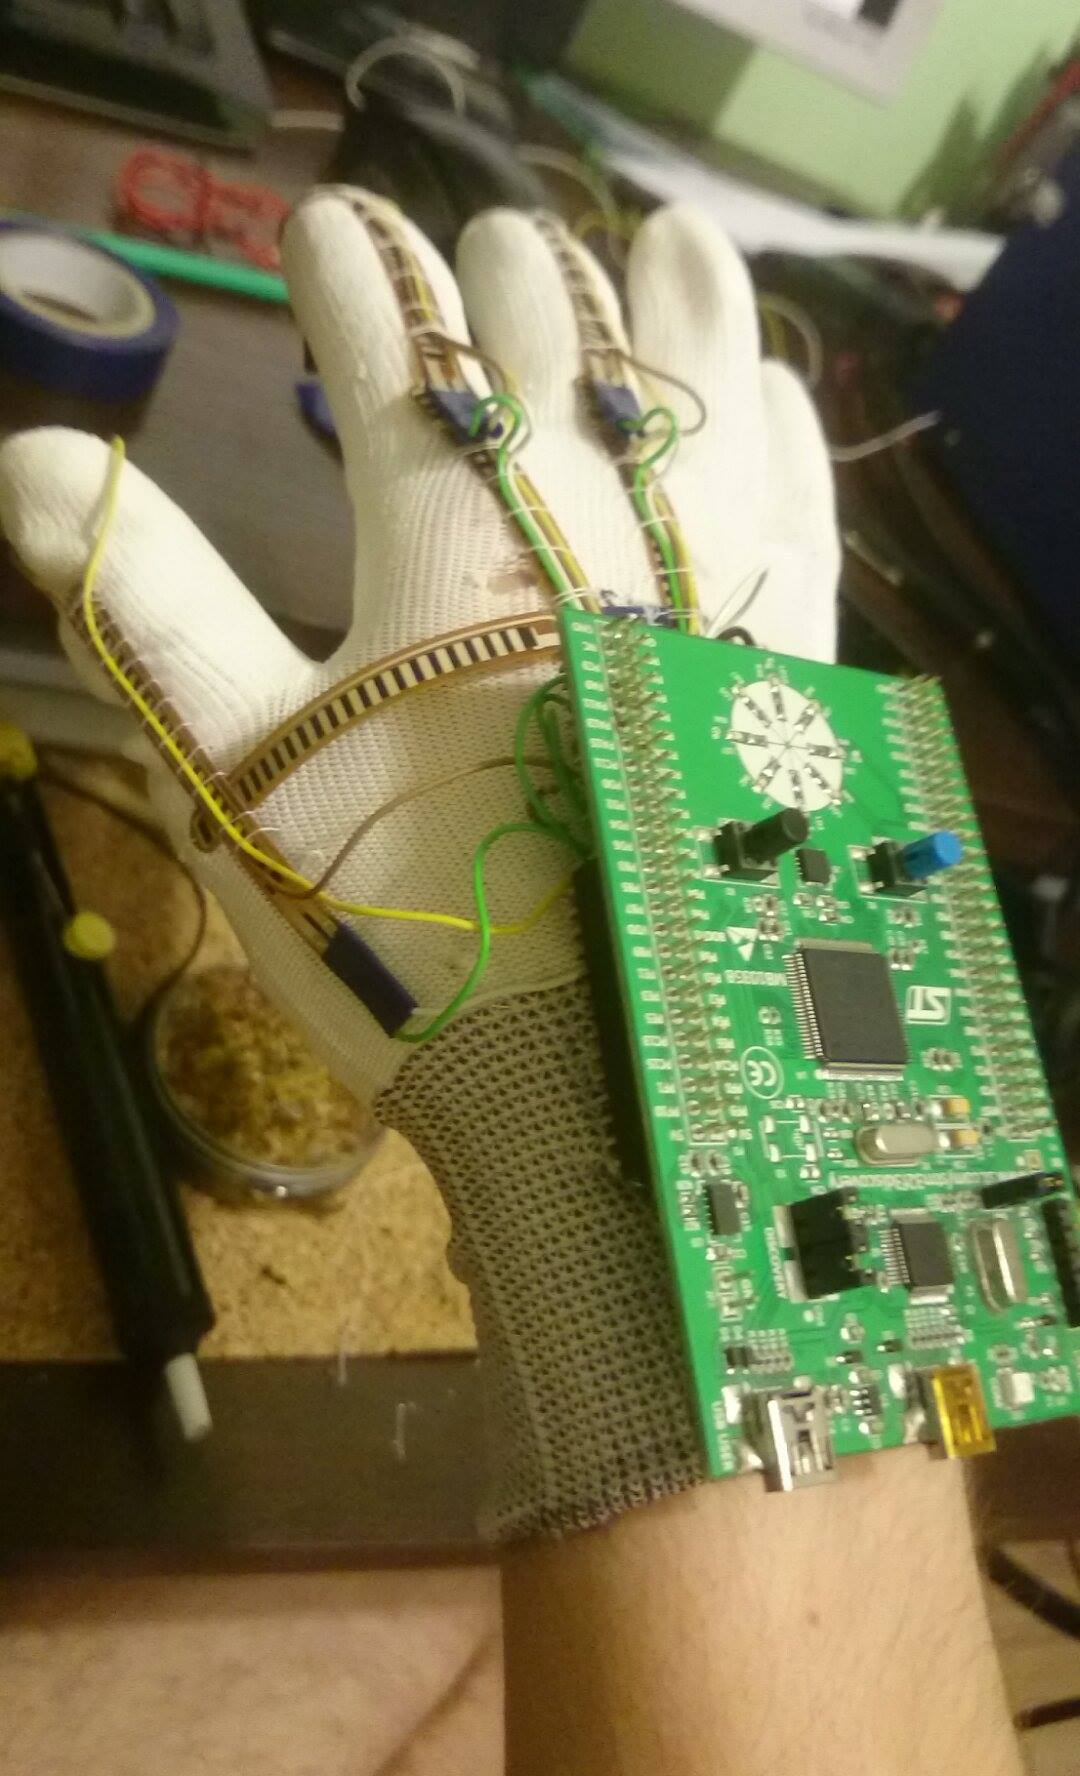
\includegraphics[width=.9\textwidth]{images/gotowa.jpg}
	\caption{Zewnętrzna część dłoni}
	\label{fig:gotowa}
\end{subfigure}%
\begin{subfigure}{.5\textwidth}
	\centering
	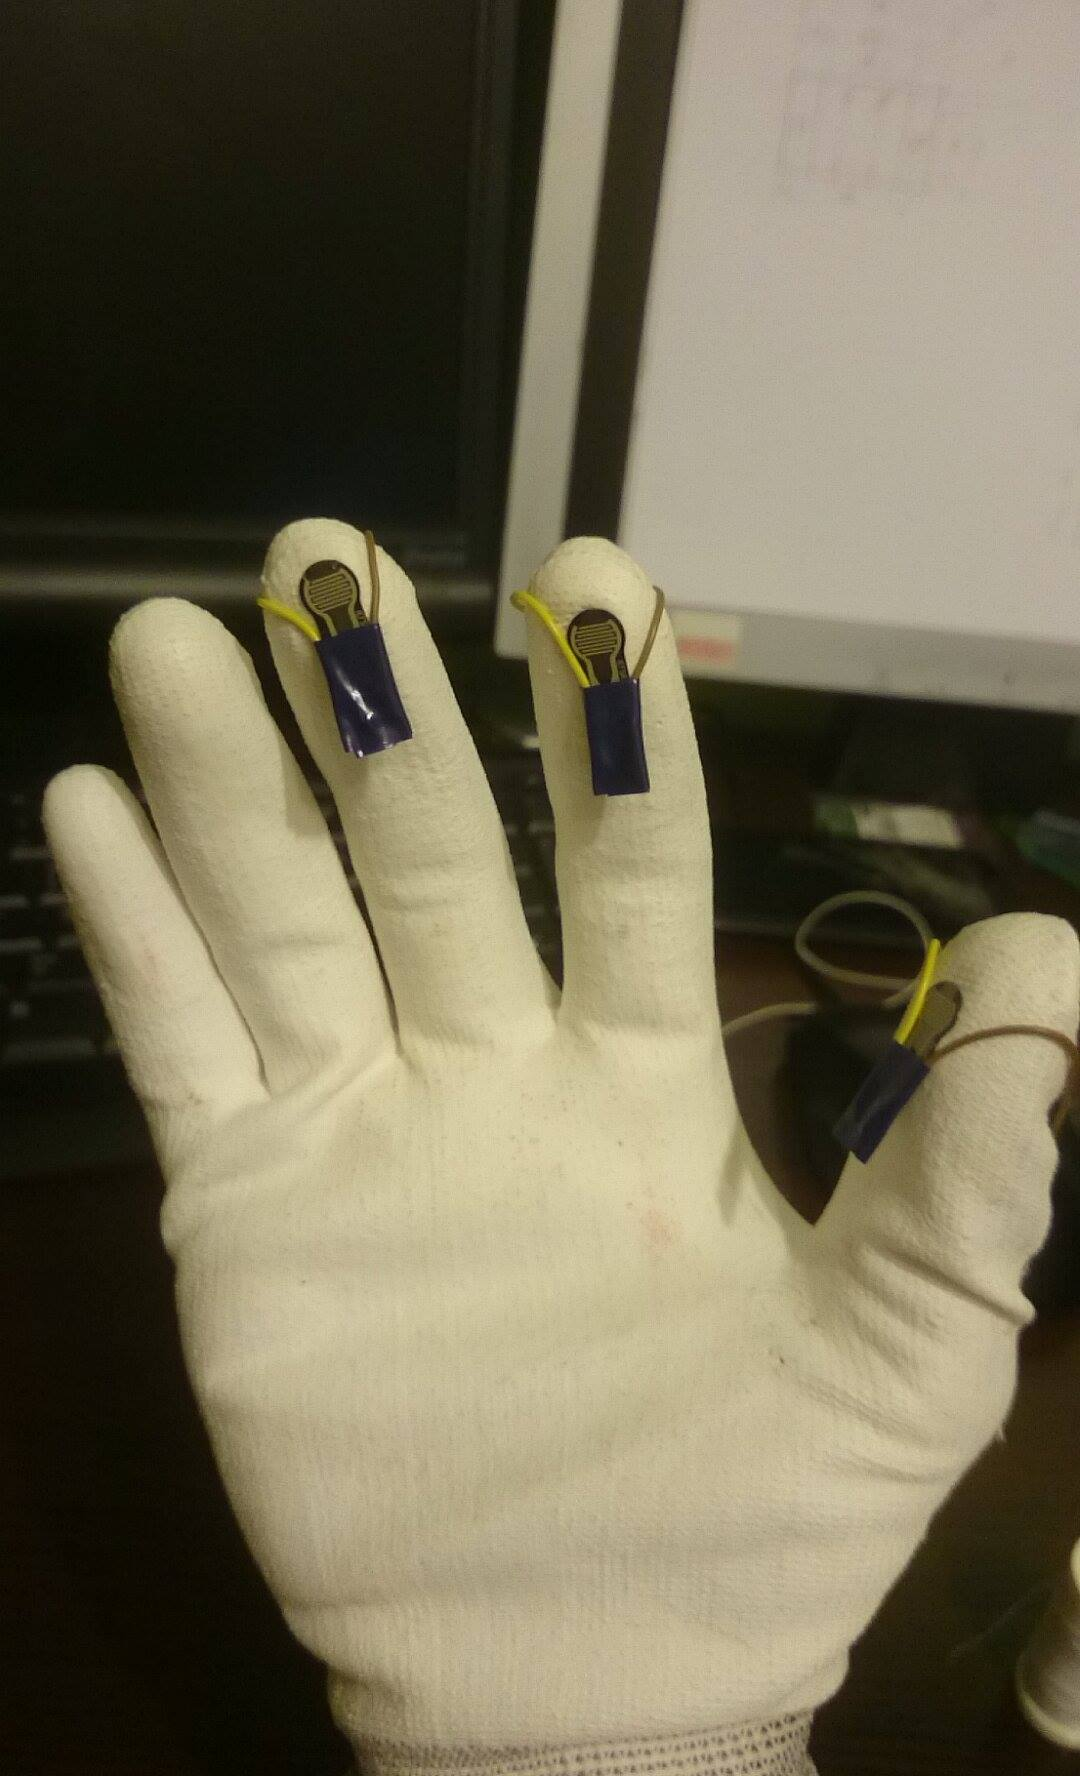
\includegraphics[width=.9\textwidth]{images/gotowa2.jpg}
	\caption{Wewnętrzna część dłoni}
	\label{fig:gotowa2}
\end{subfigure}
\caption{Gotowa rękawica}
\label{fig:gotowa_rekawica}
\end{figure}

\begin{figure}[h]
\centering
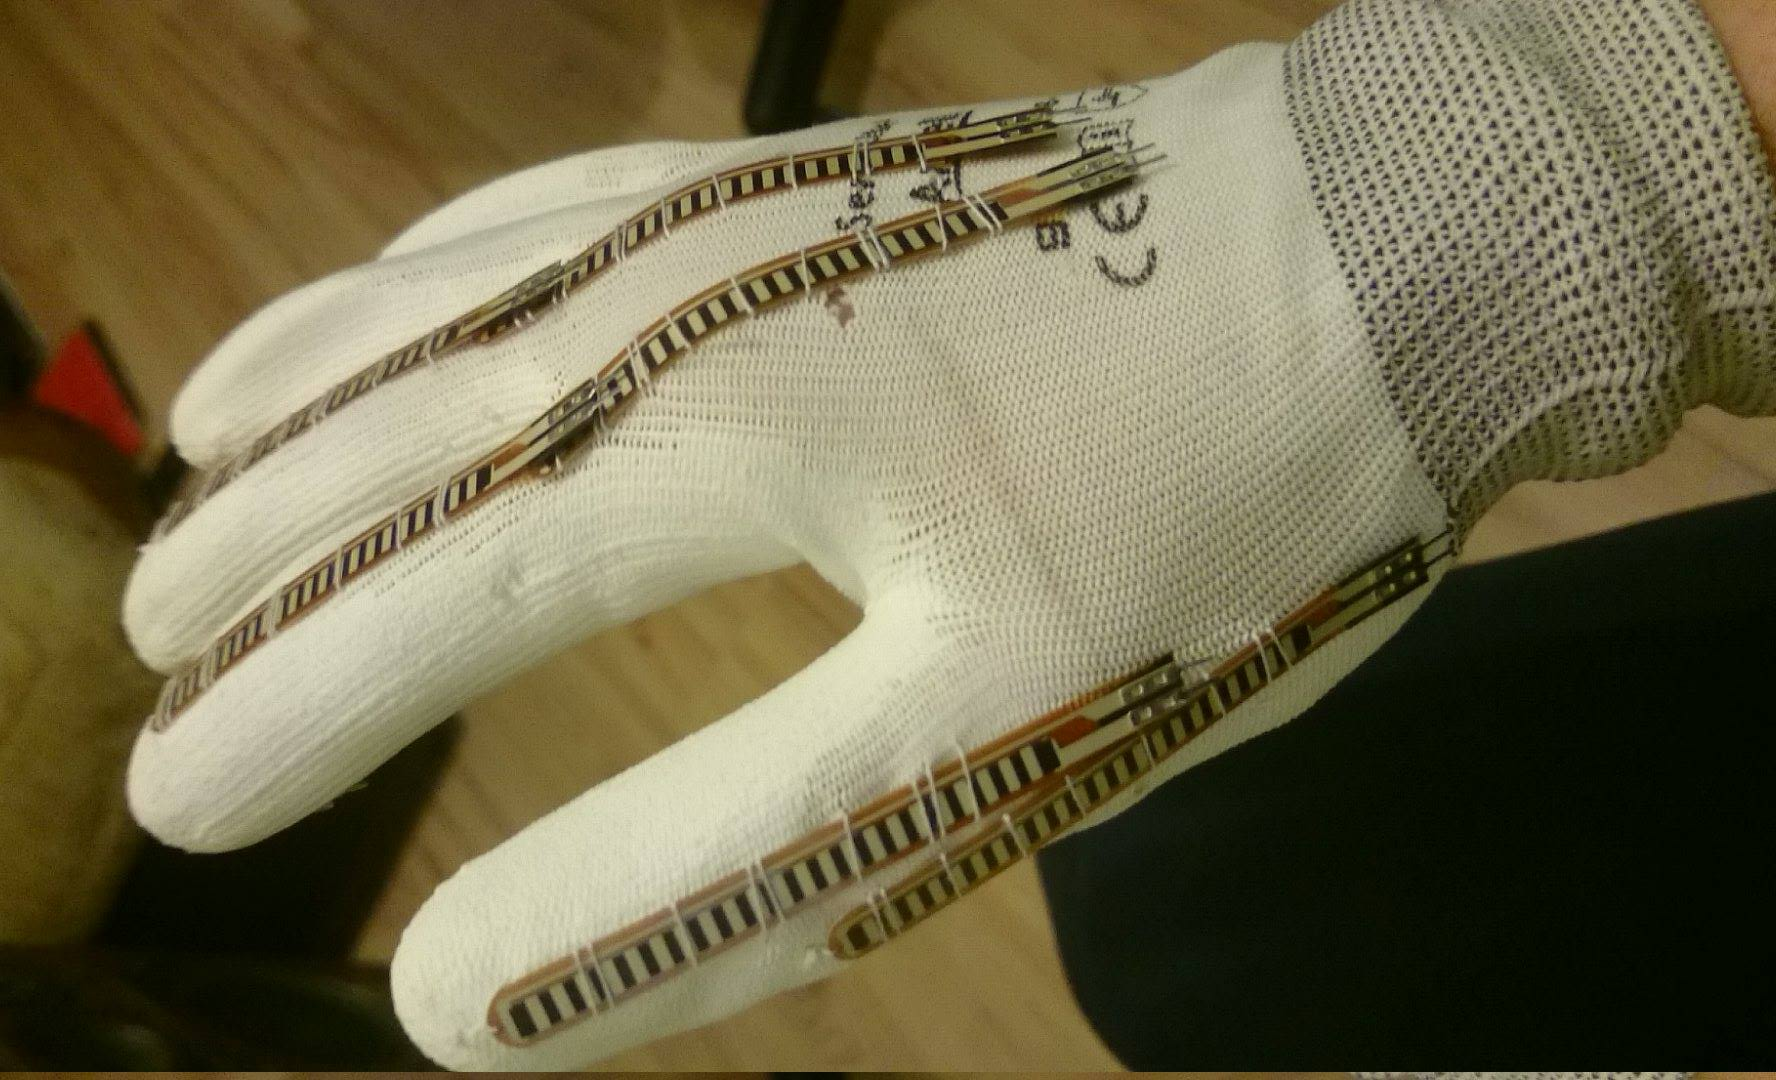
\includegraphics[width=0.65\textwidth]{images/rekawica2.jpg}
\caption{Zdjęcie rękawicy w fazie montażu (aktualny rozkład czujników jest zmieniony)}
\label{fig:rekawica2}
\end{figure}

\subsection{Testy}
Przeprowadzono testy gotowej rękawicy. Przy nacisku na czujniki na opuszkach wzrasta napięcie [rys. \ref{fig:nacisk}]. Przy zginaniu palców, czyli zgięciu flexsensorów można zabserwować wzrost napięcia w zakresie $1,35-2,8V$ [rys. \ref{fig:ugiecie}].


\subsection{Wizualizacja Danych Sensorycznych}
Powstaje aplikacja w STMStudio pozwalająca na wizualizację modelu ręki na podstawie odczytów z czujników. Aktualny interfejs graficzny wyświetla uproszczony model dłoni [rys. \ref{fig:wds}].


%\section{Podsumowanie}
%Większość prac została ukończona. Pozostało dopracowanie %prototypu rękawicy i przeprowadzenie testów w celu zebrania %pomiarów do bazy danych oraz ukończenie aplikacji do %wizualizacji danych.
\section{Krytyczna ocena działań}
Potrzebne elementy zostały zakupione z opóźnieniem. Brak kontaktu z laborantem sprawił, że przez pewien czas nie można było uzyskać informacji, czy zamówienie zostało złożone. 
\\Zgodnie z harmonogramem zostały ukończone następujące zadania:
\begin{itemize}
\item Nawiązanie łączności płytki z komputerem (USB/Bluetooth)
\item Oprogramowanie wstępnego przetwarzania danych przez płytkę
\item Przeprowadzenie wstępnych testów
\end{itemize}
Pozostałe zadania zostały wykonane ze średnio 2--tygodniowym opóźnieniem. 
\\
\begin{figure}[h]
\centering
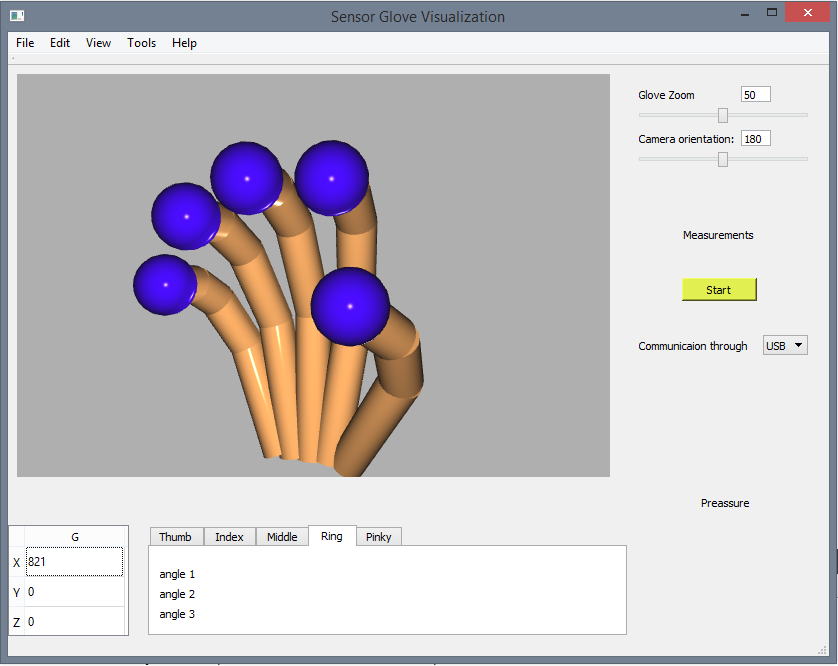
\includegraphics[width=0.8\textwidth]{images/aktualnyinterfejsgraficzny.png}
\caption{Aktualny interfejs graficzny}
\label{fig:wds}
\end{figure}

\begin{figure}[h]
\centering
\begin{subfigure}{.5\textwidth}
	\centering
	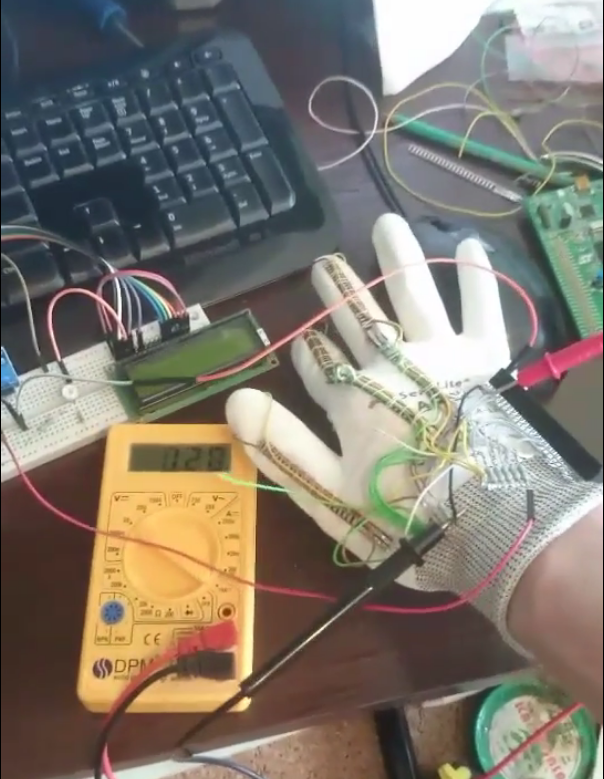
\includegraphics[width=.9\textwidth]{images/nacisk.png}
	\caption{Testowanie czujników nacisku}
	\label{fig:nacisk}
\end{subfigure}%
\begin{subfigure}{.5\textwidth}
	\centering
	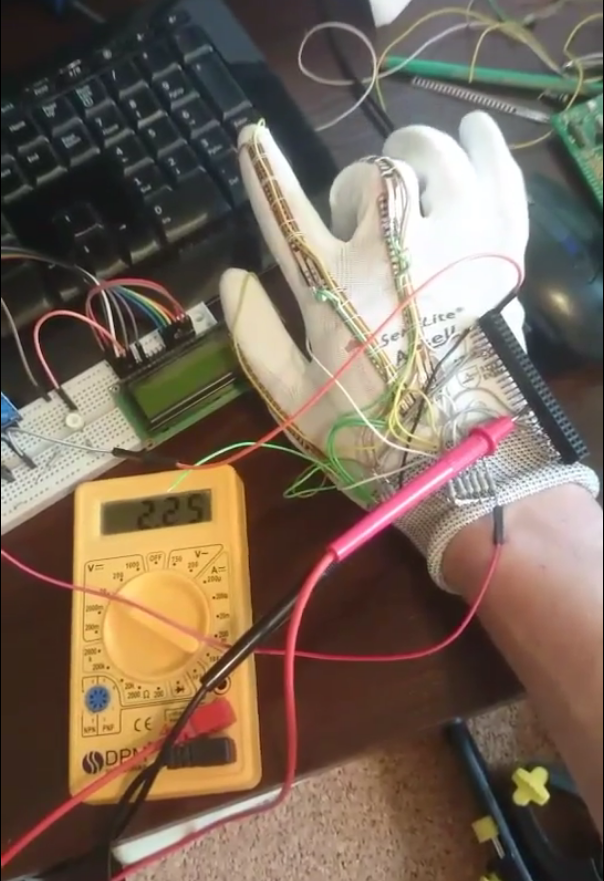
\includegraphics[width=.9\textwidth]{images/ugiecie.png}
	\caption{Testowanie czujników ugięcia}
	\label{fig:ugiecie}
\end{subfigure}
\caption{Testy}
\label{fig:testy}
\end{figure}

\end{document}
